% Chapter 4

\chapter{Evaluation} % Write in your own chapter title
\label{Chapter4}
\lhead{Chapter 4. \emph{Evaluation}} % Write in your own chapter title to set the page header

To evaluate the implementation, the SPEC2000 benchmark suite || TODO cite \\
and the Polybench/C 3.2 || TODO cite \\
suite were used to meassure correctness, applicability and speedup.


\section{The Environment}
Two computers were involved in the evaluation. The first one was a general 
purpose machine running Arch linux with an
\textit{Intel(R) Core(TM) i5 CPU M 560 @ 2.67GHz} and 6GB RAM. Parallel versions
could use up to four simultaneous running threads. 
The second one ... TODO ... 
As the compile time evaluation is machine independent, it was 
performed on the general purpose machine only. Contrary, the runtime evaluation 
has been performed twice, once on each machine. 

The work and thus the evaluation is based on an LLVM 3.0 build 
with enabled assertions and disabled optimization. All source files have been 
converted by clang to LLVM-IR files, optimized by opt and ... TODO linked TODO

\begin{center}TODO picture of the chain\end{center}


\section{Compile Time Evaluation}
The main part of the compile time evaluation aims to get quantitative results 
on the transformable code regions. These results correspond with the
applicability of this work, as they both outline how many 
regions may be transformed to increase the performance and which work is needed
to be done to raise this number. As mentioned earlier this part is machine 
independent if only these quantitative results are regarded, but there is one
case where compile time transformation can improve the program with no need of
speculation at all.
These cases are explained and evaluated separately (see section
\ref{soundCTtransformations}).

\subsection{Preperation}
TODO
 -basicaa -indvars -mem2reg -polly-independent -polly-region-simplify -polly-prepare 


\subsection{Quantitative Results}

\subsubsection{SPEC2000}
TODO why not all spec2000 benchmarks ? \\
TODO 
\begin{figure}[htbp]
	\centering
        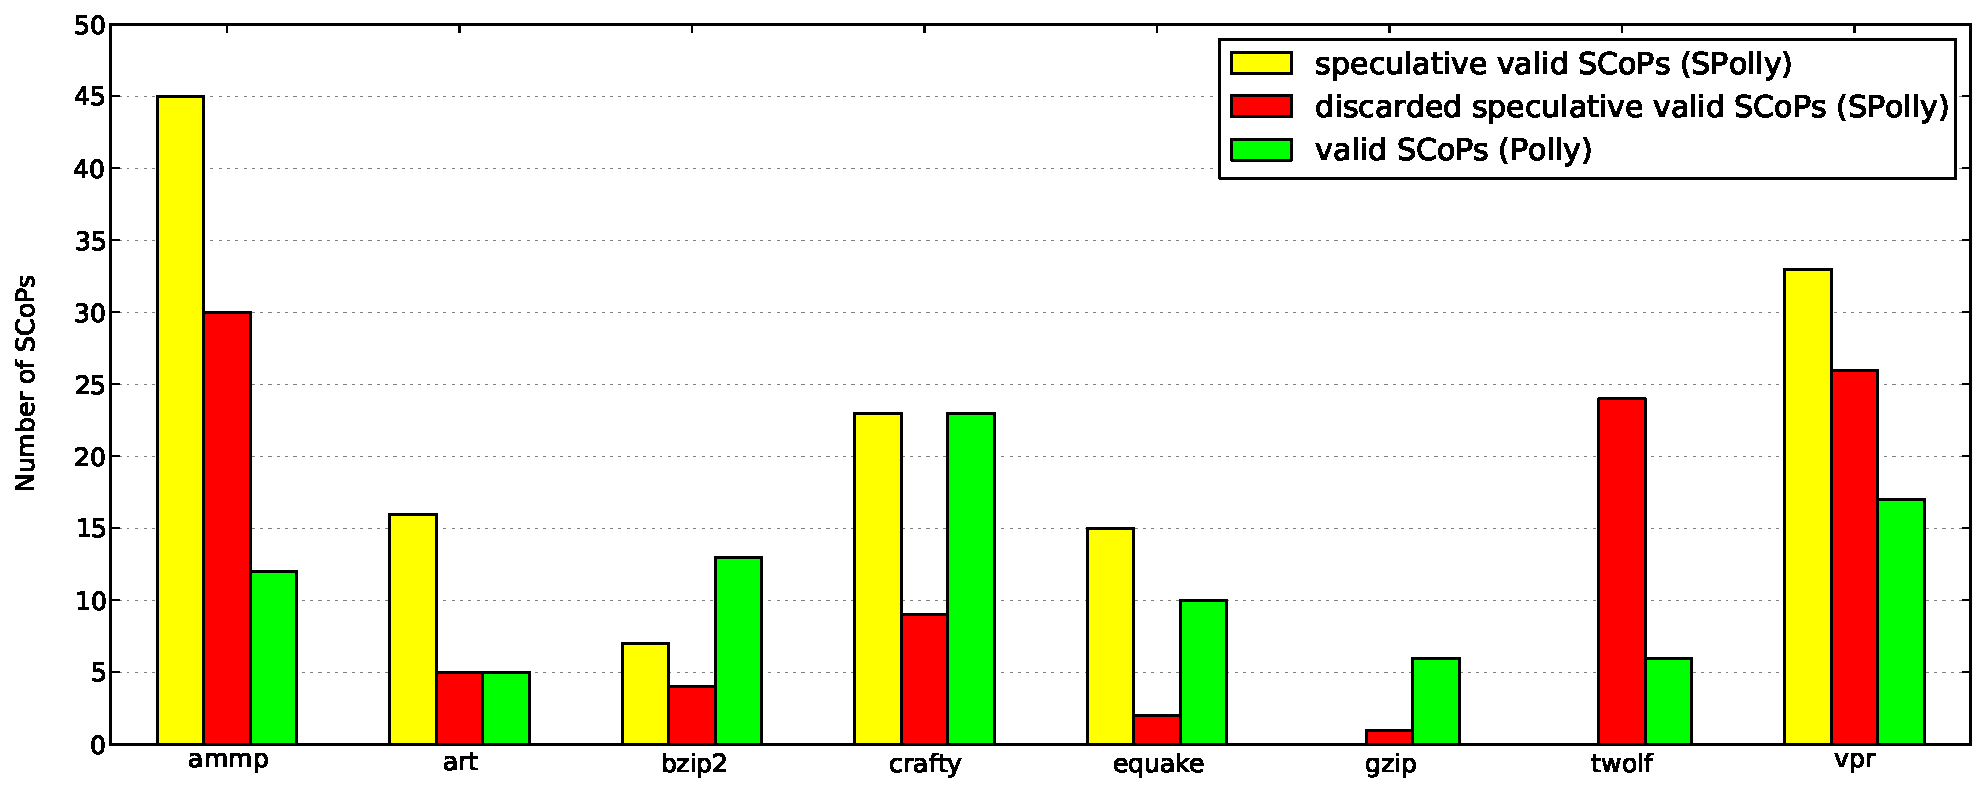
\includegraphics[width=0.9\textwidth]{SPEC2000CT.pdf}
		\rule{35em}{0.5pt}
	\caption{Numbers of valid and speculative valid SCoPs}
	\label{fig:SPEC2000CT}
\end{figure}

\subsubsection{Polybench 3.2}
\begin{figure}[htbp]
	\centering
        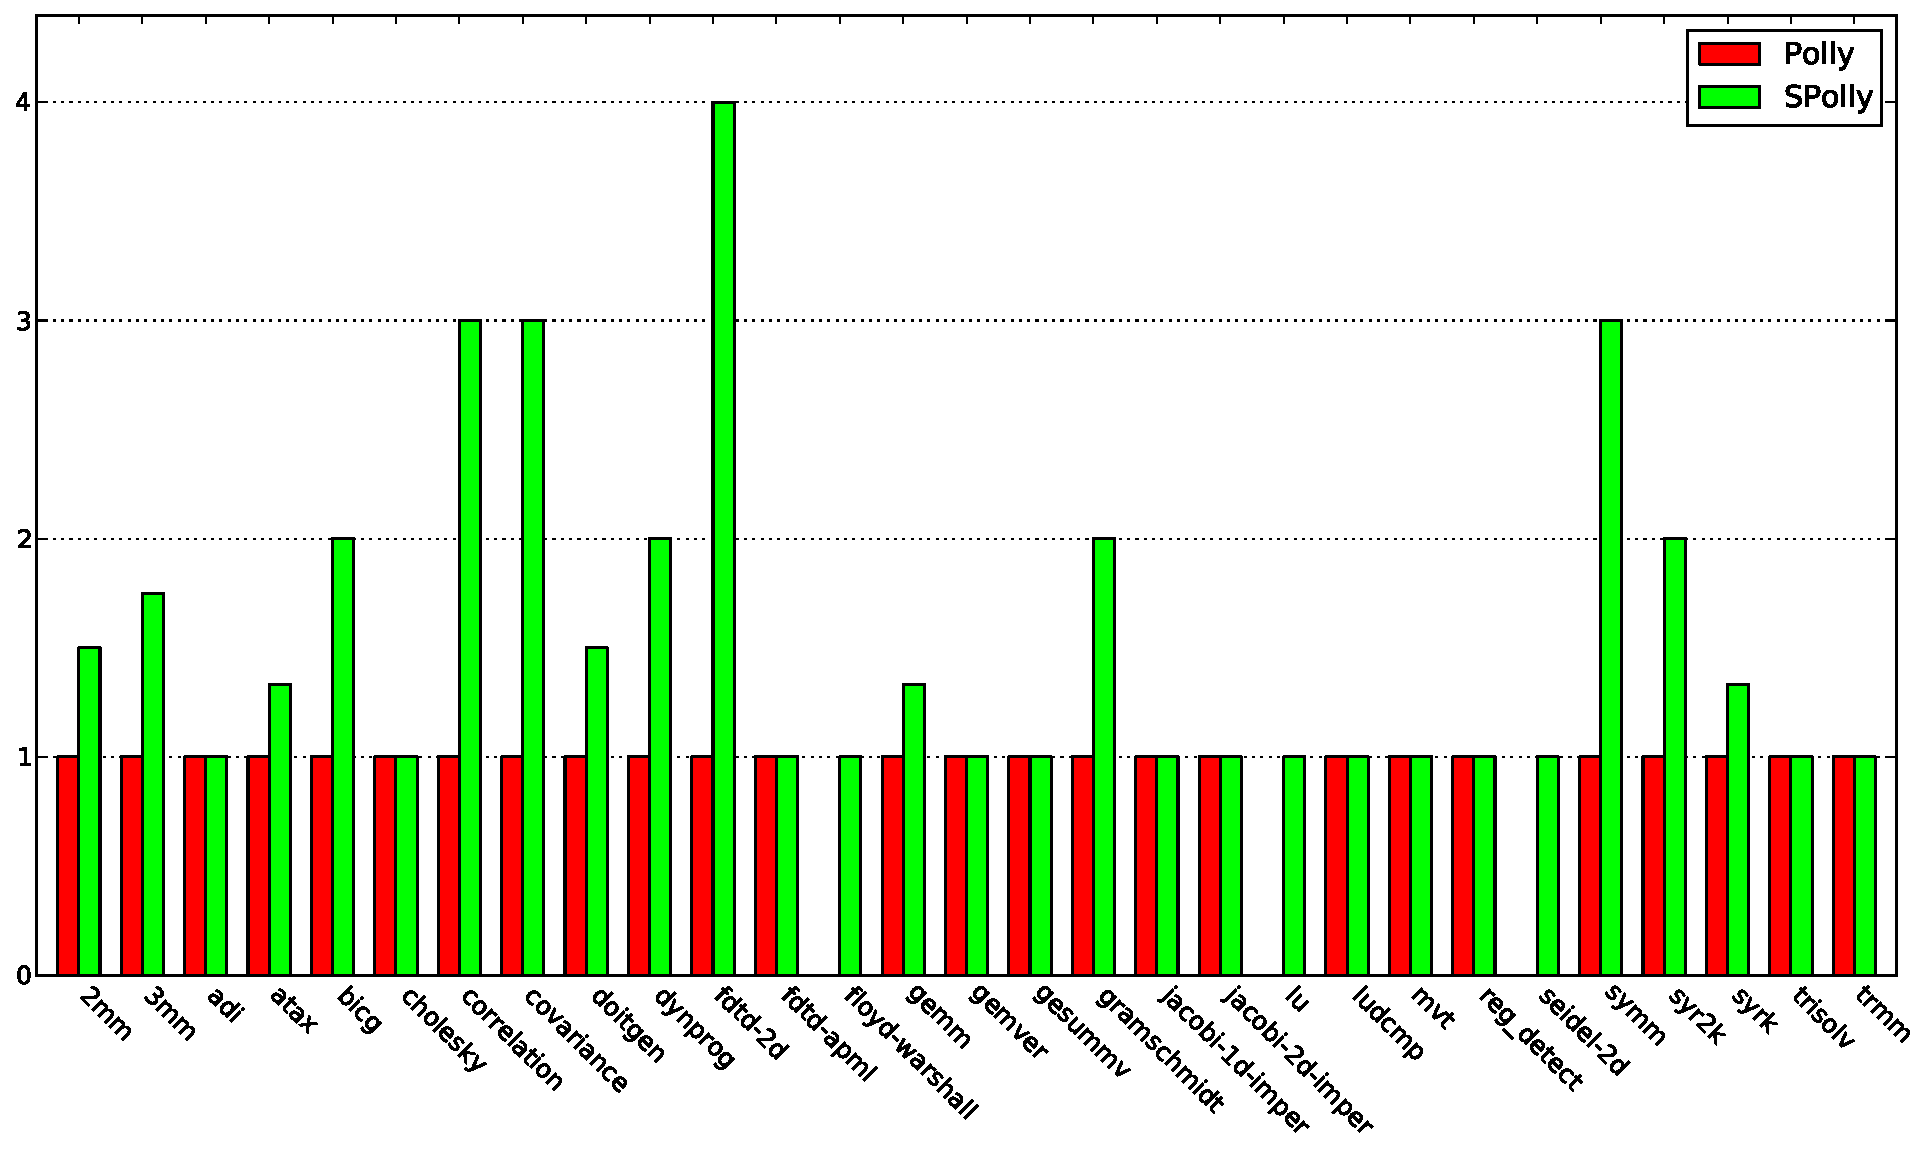
\includegraphics[width=0.9\textwidth]{polybenchCT.pdf}
		\rule{35em}{0.5pt}
	\caption{Numbers of valid and speculative valid SCoPs}
	\label{fig:polybenchCT}
\end{figure}

\begin{table}[htbp]
  \caption{Results of running Polly and SPolly on SPEC 2000 benchmarks}
  \begin{tabular}{| l | r | r | r | r | r | r | r |}
    \hline
    %\multirow{2}{*}{\textbf{Benchmark}} & \multirow{2}{*}{\textbf{\#func}} & \multicolumn{2}{c|}{\textbf{\#simple regions}} & \multirow{2}{*}{\textbf{\#instr}} &  \multicolumn{2}{c|}{\textbf{valid SCoPs}} &  \multicolumn{2}{c|}{\textbf{Avg detection time}} \\
    \multirow{2}{*}{\textbf{Benchmark}} & \multirow{2}{*}{\textbf{\#instr}} & \multicolumn{2}{c|}{\textbf{\#simple regions}} &  \multicolumn{2}{c|}{\textbf{valid SCoPs}} &  \multicolumn{2}{c|}{\textbf{Avg detec. time}} \\
    %\cline{6-9} \cline{3-4}
    \cline{3-8} 
    & & \textbf{initial} & \textbf{prepared} & \textbf{Polly} & \textbf{SPolly} & \textbf{Polly} & \textbf{SPolly} \\
    \hline
    \hline
    188.ammp   & 19824  & 205 & 208 & 12 & 45 & &  \\
    179.art    &  1667  & 66  &  66 &  5 & 16 & &  \\
    256.bzip2  &  3585  & 114 & 116 & 13 &  7 & &  \\
    186.crafty & 25541  & 305 & 310 & 23 & 23 & &  \\
    183.equake &  2585  &  70 &  71 & 10 & 15 & &  \\
    164.gzip   &  4773  &  92 &  95 &  6 &  0 & &  \\
    181.mcf    &  1663 &  33 &  33  &  0 &  0 & &  \\
    177.mesa   & 80952 & 816 & 832  & 94 &247 & &  \\
    300.twolf  & 35796 & 679 & 716  &  6 &  0 & &  \\
    175.vpr    & 19547 & 319 & 329  & 17 & 33 & &  \\
    %188.ammp   & 161 & 205 & 208 & 19824  & 12 & 45 & &  \\
    %179.art    & 22  & 66  &  66 &  1667  &  5 & 16 & &  \\
    %256.bzip2  & 59  & 114 & 116 &  3585  & 13 &  7 & &  \\
    %186.crafty & 105 & 305 & 310 & 25541  & 23 & 23 & &  \\
    %183.equake & 24  &  70 &  71 &  2585  & 10 & 15 & &  \\
    %164.gzip   & 59  &  92 &  95 &  4773  &  6 &  0 & &  \\
    %181.mcf    & 24  &  33 &  33  &  1663 &  0 &  0 & &  \\
    %177.mesa   & 769 & 816 & 832  & 80952 & 94 &247 & &  \\
    %300.twolf  & 166 & 679 & 716  & 35796 &  6 &  0 & &  \\
    %175.vpr    & 294 & 319 & 329  & 19547 & 17 & 33 & &  \\
    \hline
  \end{tabular}
\end{table}

TODO time is higher because it is SPolly/polly version not spolly only

\subsubsection{Available tests}

\paragraph{Alias tests}


\paragraph{Invariant tests}




\subsection{Sound Transformations}
\label{soundCTtransformations}
As described earlier, region speculation collects violations within a SCoP 
and can introduce tests for some of them. There are cases when these tests will
suffice to get a sound result, thus there is no need for a runtime system at all.
Although this hold in respect to the soundness of a program, this does not mean 
performance will rise when these transformations are used.  \\
TODO scores -- heuristic / statistics 


\section{Runtime Evaluation}


\section{Problems}
During the work with LLVM 3.0 and a corresponding version of Polly a few
problems occurred. Some of them could not be reproduced in newer versions
they were just be tackled with tentative fixes, as they will be resolved as soon
as Sambamba and SPolly will be ported to a newer version.
Others, which could be reproduced in the current trunk versions,
have been reported and listed in figure \ref{tab:bugreports}. All bugs were 
reported with a minimal test case and a detailed description why they occur.

% ID | description | status | patch included | tool
\begin{table}[htbp]
  \caption{Reported bugs}
  \begin{tabularx}{0.9\textwidth}{ c | X | p{2cm} | c | c }
   ID & Description & Status & Patch provided  & Component \\
  \hline \hline
  12426 & Wrong argument mapping in OpenMP subfunctions & RESOLVED FIXED & yes & Polly \\
   \hline
  12427 & Invariant instruction use in OpenMP subfunctions & NEW & yes & Polly \\
   \hline
  12428 & PHInode use in OpenMP subfunctions & NEW & no & Polly \\
   \hline
  12489 & Speed up SCoP detection & NEW & yes & Polly \\
  TODO & add the others to bugzilla & & & \\
  TODO & PollybenchC2 gemver , 2mm & & & \\
  \end{tabularx}
  \label{tab:bugreports}
\end{table}
